\documentclass[conference]{IEEEtran}
\IEEEoverridecommandlockouts
% The preceding line is only needed to identify funding in the first footnote. If that is unneeded, please comment it out.
\usepackage{cite}
\usepackage{amsmath,amssymb,amsfonts}
\usepackage{algorithmic}
\usepackage[dvipdfmx]{graphicx}
\usepackage[dvipdfmx]{color}
\usepackage{textcomp}
\usepackage{xcolor}
\usepackage{comment}
\usepackage{listings}
\usepackage{eclbkbox}
\lstset{%
  language={Java},
  basicstyle={\scriptsize},%
  identifierstyle={\scriptsize},%
  commentstyle={\scriptsize\itshape},%
  keywordstyle={\color{red}\scriptsize\bfseries},  
  ndkeywordstyle={\scriptsize},%
  stringstyle={\scriptsize\ttfamily},
  frame={tb},
  breaklines=true,
  columns=[l]{fullflexible},%
  numbers=left,%
  xrightmargin=0cm,%
  xleftmargin=0.3cm,%
  numberstyle={\scriptsize},%
  stepnumber=1,
  numbersep=0.2cm,%
  lineskip=-0.1ex%
}


\def\BibTeX{{\rm B\kern-.05em{\sc i\kern-.025em b}\kern-.08em
    T\kern-.1667em\lower.7ex\hbox{E}\kern-.125emX}}
\begin{document}

\title{SuiteRec: Automatic Test Suite Recommendation System based on Code Clone Detection\\
%{\footnotesize \textsuperscript{*}Note: Sub-titles are not captured in Xplore and
%should not be used}
%\thanks{Identify applicable funding agency here. If none, delete this.}
}


%%%%%
\author{\IEEEauthorblockN{Ryosuke Kurachi\IEEEauthorrefmark{1},  Eunjong Choi\IEEEauthorrefmark{2}, Dongsun Kim\IEEEauthorrefmark{3},Keichi Takahashi\IEEEauthorrefmark{1},  and Hajimu Iida\IEEEauthorrefmark{1}}
\IEEEauthorblockA{\IEEEauthorrefmark{1}Nara Institute of Science and Technology, Japan, \{kurachi.ryosuke.kp0, keichi\}@is.naist.jp, iida@itc.naist.jp}
\IEEEauthorblockA{\IEEEauthorrefmark{2}Kyoto Institute of Technology, Japan, echoi@kit.ac.jp\\}
\IEEEauthorblockA{\IEEEauthorrefmark{3}FuriosaAI, South Korea, darkrsw@furiosa.ai\\}
}
\maketitle

\begin{abstract}


Automatically generated tests tend to be less readable and maintainable since they often do not consider the latent objective of the target code. Reusing existing tests might help address this problem. 
To this end, we present SuiteRec, a system that recommends reusable test suites based on code clone detection. Given a java method, SuiteRec searches for its code clones from a code base collected from open-source projects, and then recommends test suites of the clones. It also provides the ranking of the recommended test suites computed based on the similarity between the input code and the cloned code. We evaluate SuiteRec with a human study of ten students. 
The results indicate that SuiteRec successfully recommends reusable test suites.


%This document is a model and instructions for \LaTeX.
%This and the IEEEtran.cls file define the components of your paper [title, text, heads, etc.]. *CRITICAL: Do Not Use Symbols, Special Characters, Footnotes, 
%or Math in Paper Title or Abstract.
\end{abstract}

\begin{IEEEkeywords}
 clone detection, recommendation system, software testing, unit test 
\end{IEEEkeywords}

\section{Introduction}
Recently, software systems have become more sophisticated and diversified, while users increasingly demand for not only ensuring software quality but also reducing costs. Software testing is one of the most important development tasks that improve software quality but it accounts for a large percentage of the total software development cost\cite{b20}. Unfortunately, most of test cases are written manually, and thus the cost will increase proportionally by the number of test cases\cite{b19}. 

To reduce the cost of writing test cases, several techniques have been proposed. 
For example, EvoSuite\cite{b3} is one of the most advanced tools for automatic unit test generation. EvoSuite statically analyzes the target code and expresses the program as symbolic values. Then, conditions that pass the control path of the target code are collected, and concrete values that satisfy the conditions are generated. By automatically generating tests, developers can save creation time and increase code coverage. 

However, automatically generated test cases are often less readable and acceptable by developers since test generation tools may not consider the development process of a given project and intention behind the target code; this can make later maintenance activities difficult\cite{b13},\cite{b14},\cite{b15}. 
% Every time a test fails, a developer has to identify the cause of the failure in the production code or determine whether the test itself needs to be updated. 
Previous studies have reported that automatically generated tests are harder to read outweigh the time-savings gained by their automated generation, and render them more of a hindrance than a help for software maintenance\cite{b1}.

In this paper, to address this problem, we propose {\sf SuiteRec}, a recommendation system to search for existing high-quality test code from open-source projects. 

The contributions from \textsf{SuiteRec} are listed below:

\noindent
$\bullet$ \textbf{Test suite recommendation using a code clone detection technique.} We propose a test-suite search method, leveraging test cases collected from open-source projects. The basic idea behind \textsf{SuiteRec} is that test cases can be reused between clone pairs. \textsf{SuiteRec} searches open-source projects for code clones of the input program and recommends test suites corresponding to the clones. The recommended test suites are ranked by their relevance. Furthermore, test smells, which indicate bad implementation of test codes, are shown for each test suite.


\noindent
$\bullet$ \textbf{Quantitative and qualitative evaluation of \textsf{SuiteRec}.} We ask human participants to write test cases with and without \textsf{SuiteRec}, and then compare the two sets of test cases to evaluate \textsf{SuiteRec}'s effectiveness. As a result, the participants can write test cases achieving a better code coverage with \textsf{SuiteRec}. In particular, the test cases written with \textsf{SuiteRec} have less test smells. In addition, the interview after the experiment show that \textsf{SuiteRec} can help participants write test code easier with high confidence.


\begin{comment}
提案ツールの評価では,被験者によってSuiteRecの使用した場合とそうでない場合でテストコードの作成してもらい,テスト作成をどの程度支援できるかを定量的および定性的に評価した.その結果,提案ツールの利用は分岐が多く複雑なプログラムのテストスイートを作成する際に,コードカバレッジを向上させることができることや,ツールを使用して作成テストコードの品質が高いことが分かった.また,定性的な評価として実験後にアンケートを実施し,推薦ツールを使った場合多くの被験者は自分の作成したテストコードに自信が持てることが分かった.
\end{comment}


We organised this paper as follows: Section~\ref{sec:background} provides the background of this study. Section~\ref{sec:suiterec} presents SuiteRec, a system that recommends reusable test suites based on code clone detection, while Section~\ref{sec:userstudy} describes a preliminary user study to evaluate \textsf{SuiteRec} and its results. After discussing related work in Section~\ref{sec:related}, we conclude the paper with future work in Section~\ref{sec:conc}.






\section{Background}
\label{sec:background}
\begin{comment}
\begin{figure*}[t]
\begin{center}
  \begin{tabular}{c}

    % 1枚目の画像
    \begin{minipage}{0.45\hsize}
      \begin{center}
\begin{lstlisting}
public class ConvertString {
    public static String convertSnakeCase(String name) {
        if (name == null) throw new NullPointerException();
        String method = name;
        Pattern p = Pattern.compile("([A-Z])");
        for (;;) {
            Matcher m = p.matcher(name);
            if (!m.find()) break;
            method = m.replaceFirst("_" + m.group(1).toLowerCase());
        }
        return method.replaceFirst("^_", "");
    }
}
\end{lstlisting}
{\scriptsize (a) Target Code fragment}
\end{center}
\end{minipage}

\hspace{0.5cm}

    % 2枚目の画像
    \begin{minipage}{0.45\hsize}
      \begin{center}
\begin{lstlisting}
public class StringUtils {
    public String toSnakeCase(String text) {
        if (text == null) throw new NullPointerException();
        String snake = text;
        Pattern p = Pattern.compile("([A-Z])");
        for (;;) {
            Matcher m = p.matcher(snake);
            if (!m.find()) break;
            snake = m.replaceFirst("_" + m.group(1).toLowerCase());
        }
        return snake.replaceFirst("^_", "");
    }
}
\end{lstlisting}
{\scriptsize (b) Similar Code fragment}
      \end{center}
    \end{minipage}
  \end{tabular}
  \end{center}
\end{figure*}

\begin{figure}[htbp]
\begin{center}
\begin{lstlisting}
public class StringUtilsTest {
    @Test(expected = NullPointerException.class)
    public void expectedExceptionfor_null() throws Exception {
    	StringUtils sut = new StringUtils();
    	sut.toSnakeCase(null);
    }
    
    @Test
    public void returnSnakeCasefor_HelloWorld() throws Exception {
     	StringUtils sut = new StringUtils();
    	String expected = "hello_world";
    	String actual = sut.toSnakeCase("HelloWorld");
        assertThat(actual, is(expected));
    }
    ...
}
\end{lstlisting}
{\scriptsize (c) Test suite for similar code fragments}
\end{center}
\end{figure}
\end{comment}


Software testing in practice still relies largely on manual tasks. Test cases are often written by developers; this includes building test harnesses, and writing test input and output pairs. Therefore, the cost of software testing is generally expensive. 

To reduce the cost, several techniques have been proposed for automated testing. The JUnit framework is one of the automated test execution tools, which makes developer focus on writing test cases. The framework provides useful functions helping test executions such as parameterized testing. Test generation tools such as EvoSuite\cite{b3} even can write test cases automatically. However, generated cases are often unable to read and maintain since the cases are generated without considering program design and user requirements. 




% In the testing phase, a developer executes test cases and see whether a target program behaves as expected in each test case. To reduce the cost of the test process, automatic test execution tools such as JUnit are widely used in the software development environment. However, test tasks are still often performed manually, and the practical application and popularization of automation technology is expected.

% Test cases developed by unit test design tasks consist of test procedures, test input values, and expected test results. The test input value is given to the software under test according to the test procedure, and the output result is compared with the expected test result. If they match, the test passes, otherwise it fails. In unit test design tasks, test input values are often developed using test case creation techniques such as equivalence partitioning and boundary analysis, but there are many variations to verify that the software works as required. You need to develop test input values for.

\begin{comment}
\textbf {Test case generation.} Existing research \cite {b12} demonstrates that existing test cases can be reused, automatically generated, or reapplied to save significant time and money in the software development testing process. It shows. There are five main test generation techniques: random test (RT), symbol execution (SE), search base test (SBST), model base (MBT), and combination test. SE is further divided into static symbol execution (SSE) and dynamic symbol execution (DSE).

RT is a test method that gives random input to the software. Random tests that run randomly and uniformly are suitable for automation, but the efficiency per test case is extremely poor in terms of improving code coverage and bug detection.

SE analyzes the target code statically, expresses the program as a symbolic value, extracts the conditions corresponding to each path in the code, and collects the conditions that the input values that pass through the path must satisfy. For each path, the conditions are solved using a constraint solver such as the SMT solver [5], and the obtained concrete value is used as the test input value.

SBST is a generic name for technologies that generate test suites that satisfy the requirements to be achieved using a heuristic search algorithm based on an evaluation function designed to quantitatively evaluate the degree of achievement for the requirements to be achieved.

MBT is a general term for technologies that generate test suites based on models. The model describes the target in some form. The model for requirements analysis and design may be used, or the model may be developed for testing.

CT is a method of generating combinations of values assigned to parameters as test cases in order to effectively find defects caused by interaction between parameters.
\end{comment}

% \textbf{Unit testing. }単体テストの実行タスクでは,ソフトウェアを動作させ,それぞれのテストケースにおいてソフトウェアが期待通りの振る舞いをするかを確認する.テスト工程のコスト削減のため,テスト実行タスクにおいて,単体テストではJUnitなどのテスト自動実行ツールの利用が産業界で進んでいる.しかし,テスト設計タスクは未だ手動で行うことが多く,自動化技術の実用化および普及が期待されている.

% 単体テスト設計タスクで作成されるテストケースは,テスト手順,テスト入力値,テスト期待結果から構成される.テスト手順に従ってテスト対象のソフトウェアにテスト入力値を与え,その出力結果をテスト期待結果と比較する.これが一致していればテストは合格となり,一致しなければ不合格となる.単体テスト設計タスクにおいては,多くの場合同値分割法,境界地分析法などのテストケース作成技法を用いてテスト入力値を作成するが,ソフトウェアの要求通りに動作するかを確認するために多くのバリエーションのテスト入力値を作成する必要がある.

% \textbf{Test case generation. }既存の研究\cite{b12}は,既存のテストケースを再利用,自動生成,または再適用できることによって,ソフトウェア開発のテスト工程における時間とコストを大幅に節約できることを示している.テスト生成技術は,主にランダムテスト(RT),記号実行(SE),サーチベーステスト(SBST),モデルベース(MBT),組み合わせテストの5つに分類できる.SEはさらに静的記号実行(SSE)と動的記号実行(DSE)に分けられる.

% RTとは,ソフトウェアにランダムな入力を与えるテスト手法である.無造作・均一にテストを実行するランダムテストは自動化に適しているが,コードカバレッジ率向上,バグ検出の観点において,テストケース1件当たりの効率は著しく悪い.

% SEは対象コードを静的解析してプログラムを記号値で表現し,コード上のそれぞれのパスに対応する条件を抽出し,パスごとにパスを通るような入力値が満たすべき条件を集める.そして,パスごとにその条件をSMTソルバ[5]などの制約ソルバを用いて解き,得られた具体値をテスト入力値とする.

% SBSTは,達成したい要件に対する達成度合いを定量的に評価できるように設計した評価関数に基づいて,ヒューリスティック探索アルゴリズムを用いて達成したい要件を満足するテストスイートを生成する技術の総称である.

% MBTはモデルに基づいてテストスイートを生成する技術の総称である.モデルは何らかの形でテスト対象を記述したものであり,要求分析や設計のためのモデルを活用することもあれば,テストのためにモデルを作成することもある.

% CTは,パラメータ間の相互作用に起因する不具合を効果的に発見するためにテストケースとしてパラメータに割り当てる値の組み合わせを生成する手法である.

\textbf{Test Smell.} The importance of well-designed test code was initially emphasized by Beck\cite{b4}. Beck argued that test cases following good design principles are desirable since they are easier to understand, maintain, and can be successfully used to diagnose problems in a program. Inspired by these arguments, van Deursen et. al.,\cite{b7} coined the test smells and defined the first catalog of 11 poor design choices to write tests, together with refactoring operations aimed at removing them. Such a catalog has been then extended more recently by practitioners, such as Meszaros\cite{b6} who defined 18 new test smells. As reported by recent studies, their presence might not only negatively affect the comprehension of test suites but can also lead to test cases being less effective in finding bugs in production code\cite{b8}.

\section{SuiteRec}
\label{sec:suiterec}
%\textsf{SuiteRec} takes a code fragment from the developer and searches in exsiting OSS projects to identify test suites that are correspond to the developer’s input. Furthermore, test smells in test suites are detected, and test suites are ranked in descending order of quality.
\textsf{SuiteRec} searches for similar methods to a given Java method by using a code clone detection tool. It then recommends test suites of the similar methods based on test smells and similarity between the given and similar methods. Figure~\ref{fig1} shows the main steps of \textsf{SuiteRec} for recommending test suites. The main steps consists of the following four steps:


\begin{figure}[htbp]
\centerline{\includegraphics[width=8.5cm]{SuiteRec-outline.pdf}}
\caption{Overview of \textsf{SuiteRec}.}
\label{fig1}
\end{figure}



\begin{enumerate}
\renewcommand{\labelenumi}{(\arabic{enumi})}
\item \textbf{ Code Clone Detection:} given an input Java method \textit{m}, it searches a source code database for a set of $m$'s similar code fragments by using an existing clone detection tool.
\item \textbf{Test Code Detection:} identifies a set of test suites of similar code fragments from a test code database.
\item \textbf{Test Smell Detection:} identifies a set of test smells from test suites using a test smell detection tool.
\item \textbf{Test Suites Recommendation: } ranks test suites  based on test smells and similarity between $m$ and source code of the test suites.
\end{enumerate}



\subsection{Code Clone Detection}
The goal of this step is to identify cloned code of a given input method \textit{m} from OSS projects. In this step, at first, it detects clone pairs using \textsf{NiCad}\cite{b2} between the input code \textit{m} and a source code database. \textsf{NiCad} is selected because it has been widely used in the clone detection community and it has a both high precision and high recall. We use the default settings of \textsf{NiCad} (i.e., each clone pair has more than 70\% of similarity and the clones contain at least 10 lines of code). The source code database contains source code from 3,205 selected GitHub projects. The selected projects contain test folders in the projects and adopted the JUnit testing framework. To seed up detection time of clone pairs, large-scale projects were divided, small-scale projects were integrated, and multiple detection processes were run in parallel, which makes  detection faster. From the detected clone pairs, we identifies all clone pairs $\left(c_{i}, m\right) $.


\begin{table*}[t]
\caption{Six Relevant Test Smells for Reusing Test Suites.}
\label{smells}
\begin{tabular}{|l|p{14.5cm}|}
\hline
\textbf{Name}                   & \textbf{Description}                                                                                                       \\ \hline
\textbf{Assetion Roulette}        & Occurs when a test method has multiple assertions. Multiple assertion statements in a test method without a descriptive message impacts readability/understandability/maintainability as it’s not possible to understand the reason for the failure of the test.  \\ \hline
\textbf{Conditional Test Logic} & Test methods need to be simple and execute all statements in the production method. Conditional code with in a test method negatively impacts the ease of comprehension by developers.\\ \hline
\textbf{Default Test}            & Test code in which the test class or test method name is the default in test code using a testing framework such as JUnit. It is necessary to change the name appropriately to improve the readability of the code.                                                                                                      \\ \hline
\textbf{Eager Test }             & Occurs when a test method invokes several methods of the production object. This smell results in difficulties in test comprehension and maintenance. \\ \hline
\textbf{Exception Handling}      & This smell occurs when a test method explicitly a passing or failing of a test method is dependent on the production method throwing an exception. Developers should utilize JUnit's exception handling to automatically pass/fail the test instead of writing custom exception handling code or throwing an exception. \\ \hline
\textbf{Mystery Guest}          & Occurs when a test method utilizes external resources (e.g., files, database). Use of external resources in test methods will result in stability and performance issues. Developers should use mock objects in place of external resources. \\ \hline
\end{tabular}
\end{table*}

\subsection{Test Code Detection}
The goal of this step is to identify test cases of cloned code $c_i$. To do this, we created traceability links between source code and its test case and then stored this information to a test code database as follows:

%e fragments. In this research, the following two steps are taken in order to precisely link the target code with test code fragments.
%In order to search for test suites correslar code fragments, the target code is linked with test code fragments. In this research, the following two steps are taken in order to precisely link the target code with test code fragments.

%\begin{figure}[htbp]
%\centerline{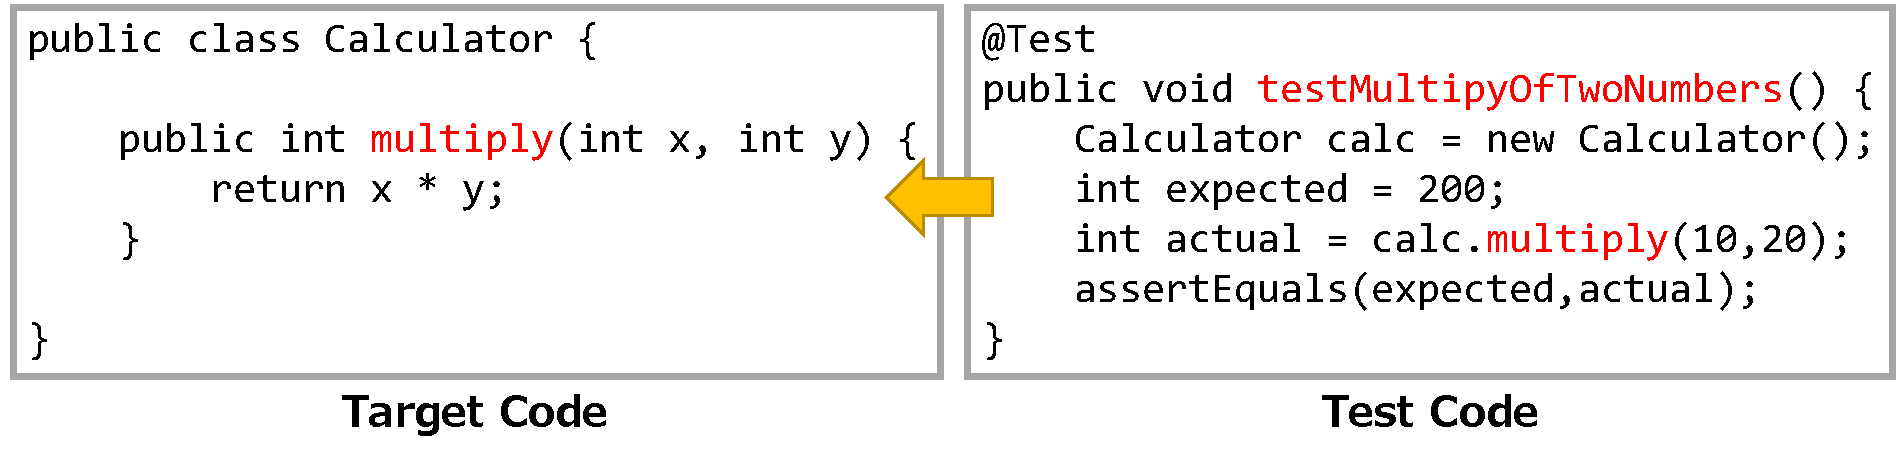
\includegraphics[width=8.5cm]{mapping.pdf}}
%\caption{Example of creating a traceability link between source code and test code}
%\label{fig2}
%\end{figure}

\begin{enumerate}
\renewcommand{\labelenumi}{(\arabic{enumi})}
\item  Collect all method names which are called from each test case.
\item  Split a name of each test code by a delimiter or between the camelcase words.
\item  Create a traceability link between test code and source code if the splitted test code name particularly match with the callee method names.
\end{enumerate}

Generally, it is recommended to use a name that express what we expected to test for a test method. The name of the target method is often described in the test method name\cite{b22}. Therefore, we used names of source code and test code to create the links. From the test code data base where the linkes are stored, this step identifies links between test cases and cloned code $c_i$. 

%\begin{enumerate}
%\renewcommand{\labelenumi}{(\arabic{enumi})}
%\item Statically analyze the test code and obtain the method call of the target code.
%\item Divide the test method with a delimiter or capital letter and link it when the target method partially matches.
%\end{enumerate}

%In the unit test, the target object is generated in the test code as shown in the figure \ref{fig2}, and it is executed by calling a method of the target code. Therefore, to link the target code to the test code, the test code in the Test Code Database is statically analyzed and the method call is obtained. However, multiple methods may be called within one test method, so the method names are also compared. It is recommended to faithfully represent the contents of the processing of the target method as the test method name description method, and the name of the target method is often described in the test method name\cite{b22}. Therefore, the name of the test method is divided by a delimiter or capital letter, and it is linked if it partially matches the target method.

%The Test Code Database in Figure \ref{fig1} stores test code corresponding to the production code in The Source Code Database. As a pre-processing, static analysis was performed on large-scale projects in advance, and information that linked target code and test code was stored in the DB, so that test code could be searched at high speed via the DB.

\subsection{Test Smell Detection}
The goal of this step is to detect test smells from the test suites. To this end, \textsf{tsDetect}\footnote{http://testsmells.github.io} was adopted as a test smell detection tool \cite{b9}. \textsf{tsDetect} is an AST-based tool that detects 19 test smells. It is also know for high accuracy to detect test smells (i.e., 85\% to 100\% accuracy and 90\% to 100\% recall). 

Among 19 detectable test smells, we determined that following four code smells as indicators of inappropriate test smells for reusing. 

\begin{itemize}
\item \textbf{Empty Test} occurs when a test method does not contain executable statements.
\item \textbf{Ignored Test} indicates that test code has the @Ignore annotation and could not be executed.
\item \textbf{Redundant Assertion} occurs when test methods contain assertion statements that are either always true or always false. 
\item \textbf{Unknown Test} shows that a test method that does not contain a single assertion statement.
\end{itemize}

Therefore, we excluded test suites that contain above-mentioned four test smells from the test code database. Moreover, we also choose six test smells that provide valuable information for reusing. Table \ref{smells} shows the detailed information of these six smells. 




\begin{comment}

\begin{table}[hbtp]
\caption{Six Test Smells}
\begin{tabular}{|l|p{5.2cm}|}
\hline
\textbf{Name}                   & \textbf{Description}                                                                                                       \\ \hline
\textbf{Assetion Roulette}        & Occurs when a test method has multiple non-documented assertions. Multiple assertion statements in a test method without a descriptive message impacts readability/understandability/maintainability as it’s not possible to understand the reason for the failure of the test.  \\ \hline
\textbf{Conditional Test Logic} & Test methods need to be simple and execute all statements in the production method. Conditions within the test method will alter the behavior of the test and its expected output, and would lead to situations where the test fails to detect defects in the production method since test statements were not executed as a condition was not met. Furthermore, conditional code within a test method negatively impacts the ease of comprehension by developers. \\ \hline
\textbf{Default Test}            & Test code in which the test class or test method name is the default in test code using a testing framework such as JUnit. It is necessary to change the name appropriately to improve the readability of the code.                                                                                                      \\ \hline
\textbf{Eager Test }             & Occurs when a test method invokes several methods of the production object. This smell results in difficulties in test comprehension and maintenance. \\ \hline
\textbf{Exception Handling}      & This smell occurs when a test method explicitly a passing or failing of a test method is dependent on the production method throwing an exception. Developers should utilize JUnit's exception handling to automatically pass/fail the test instead of writing custom exception handling code or throwing an exception. \\ \hline
\textbf{Mystery Guest}          & Occurs when a test method utilizes external resources (e.g., files, database). Use of external resources in test methods will result in stability and performance issues. Developers should use mock objects in place of external resources. \\ \hline
\end{tabular}
\end{table}

\end{comment}





\subsection{Test Suites Recommendation}
The goal of this step is to rank test suites based on the similarity and quality of test suites. \textsf{SuiteRec} ranks test suites based on similarity between source code and input code and the number of test smells contained in the test suites. 
Generally, more similar source code likely to be more similar in test code. Thus, test suites of more similar code to the input code might provide a clue to developers how to reuse existing test suites. Therefore, at first, it ranks the test suites according to similarity between the input code and source code of the test suites. Furthermore, test suites with more smells indicate that they have a high risk of bugs or failures in the future. Therefore, it ranks the test suites based on the number of test smells in the test suites. In other words, test suites whose source code is more similar to the input code with less test smells ranks higher than other test suites. 
Figure \ref{fig:screen} shows how \textsf{SuiteRec} recommends test suites with relevant information for reusing test suites as follows:


\begin{figure*}[htbp]
\centerline{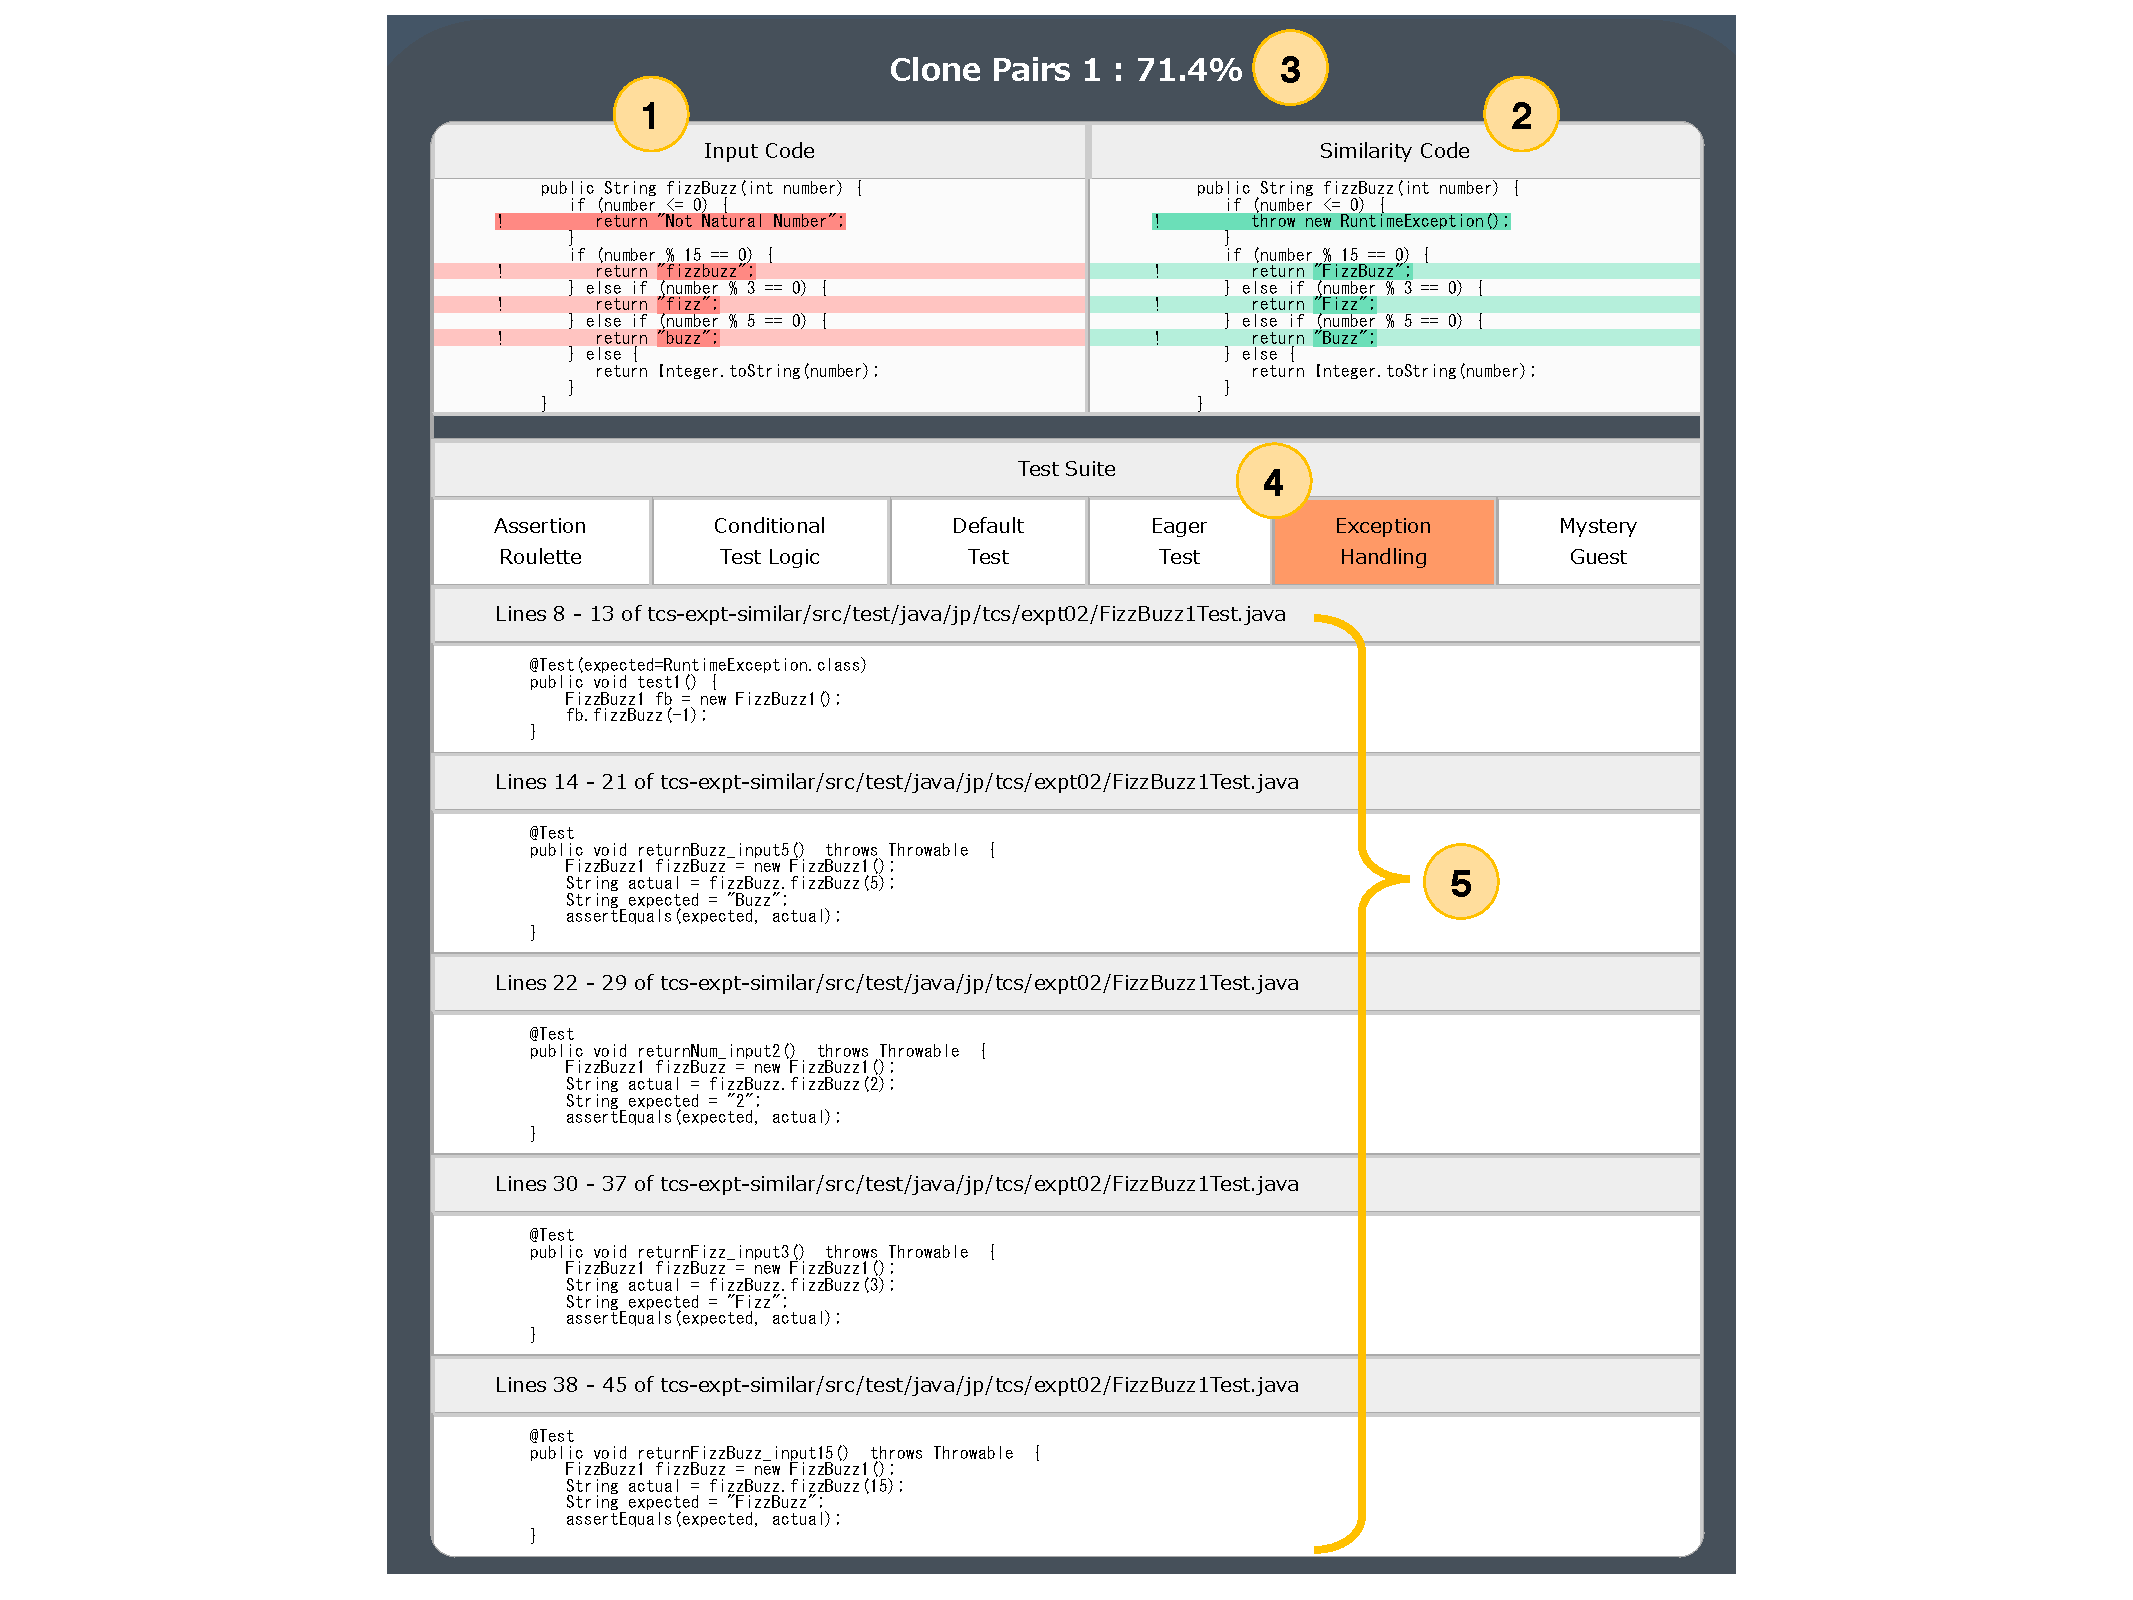
\includegraphics[width=18cm]{SuiteRec.pdf}}
\caption{Screenshot of \textsf{SuiteRec}.}
\label{fig:screen}
\end{figure*}


\begin{enumerate}
\renewcommand{\labelenumi}{(\arabic{enumi})}
\item{\textbf{Input Code:} The target code for generating test suites (i.e., input code) is displayed.}
\item{\textbf{Similarity Code fragment:} Each similar code to the input code is displayed. Moreover, the differences between input code and similar code are highlighted in order to make developers easily understand similar code and its context.}
\item{\textbf{Degree of similarity:} The similarity between the input code fragment and the similar code fragment is displayed. The similarity is calculated using the Unique Percentage of Items (UPI) method used by \textsf{NiCad}.}
\item{\textbf{Test Smells:} If test smells are contained in the test suite, test smells are highlighted with an orange color, so that developers can readily understand the existence of test smells in the displayed test suites.}
\item{\textbf{Recommend Test Suites:} The code of recommended test suite is displayed with a file path information to represent information of OSS projects where the test suite is belonging. }
\end{enumerate}


\section{Preliminary User Study}
\label{sec:userstudy}
To quantitatively and qualitatively evaluate \textsf{SuiteRec}, we conducted a preliminary user study with 10 students developers, aiming at answer the following four research question(RQ)s:

\begin{itemize}
\item \textbf{RQ1. How well can \textsf{SuiteRec} support generating test suites with high code coverage?} Code coverage is an important indicator of how well the software has been tested. We set up this RQ to confirm whether \textsf{SuiteRec} can contribute to increasing quality of the software.
\item \textbf{RQ2. How well can \textsf{SuiteRec} reduce test suites generate time?} Generally, it takes much time to generate test suites from scratch. We set up this RQ to confirm whether \textsf{SuiteRec} can contribute to shorten the test suites generation time.
\item \textbf{RQ3. How well \textsf{SuiteRec} support generate test code with high quality?} We set up this RQ to confirm whether \textsf{SuiteRec} can contribute to generating high-quality test code (i.e., with a fewer test smells).
\item \textbf{RQ4. How effective \textsf{SuiteRec} is to support test suites generation tasks?} We set up this RQ to confirm how well \textsf{SuiteRec} can support developers in generating test suites.
\end{itemize}





\subsection{Setup}
For the preliminary user study, we recruited students who have basic programming skills and software testing knowledge. The user study was conducted with 10 master course students who majored in information science. Among participants, more than 90\% of participants had more than two years of programming experience, and more than 80\% of participants had more than one year of Java language experience. All participants had a basic knowledge about software testing, and more than 80\% had experience in developing unit tests.





 \begin{figure}[htbp]
 \centerline{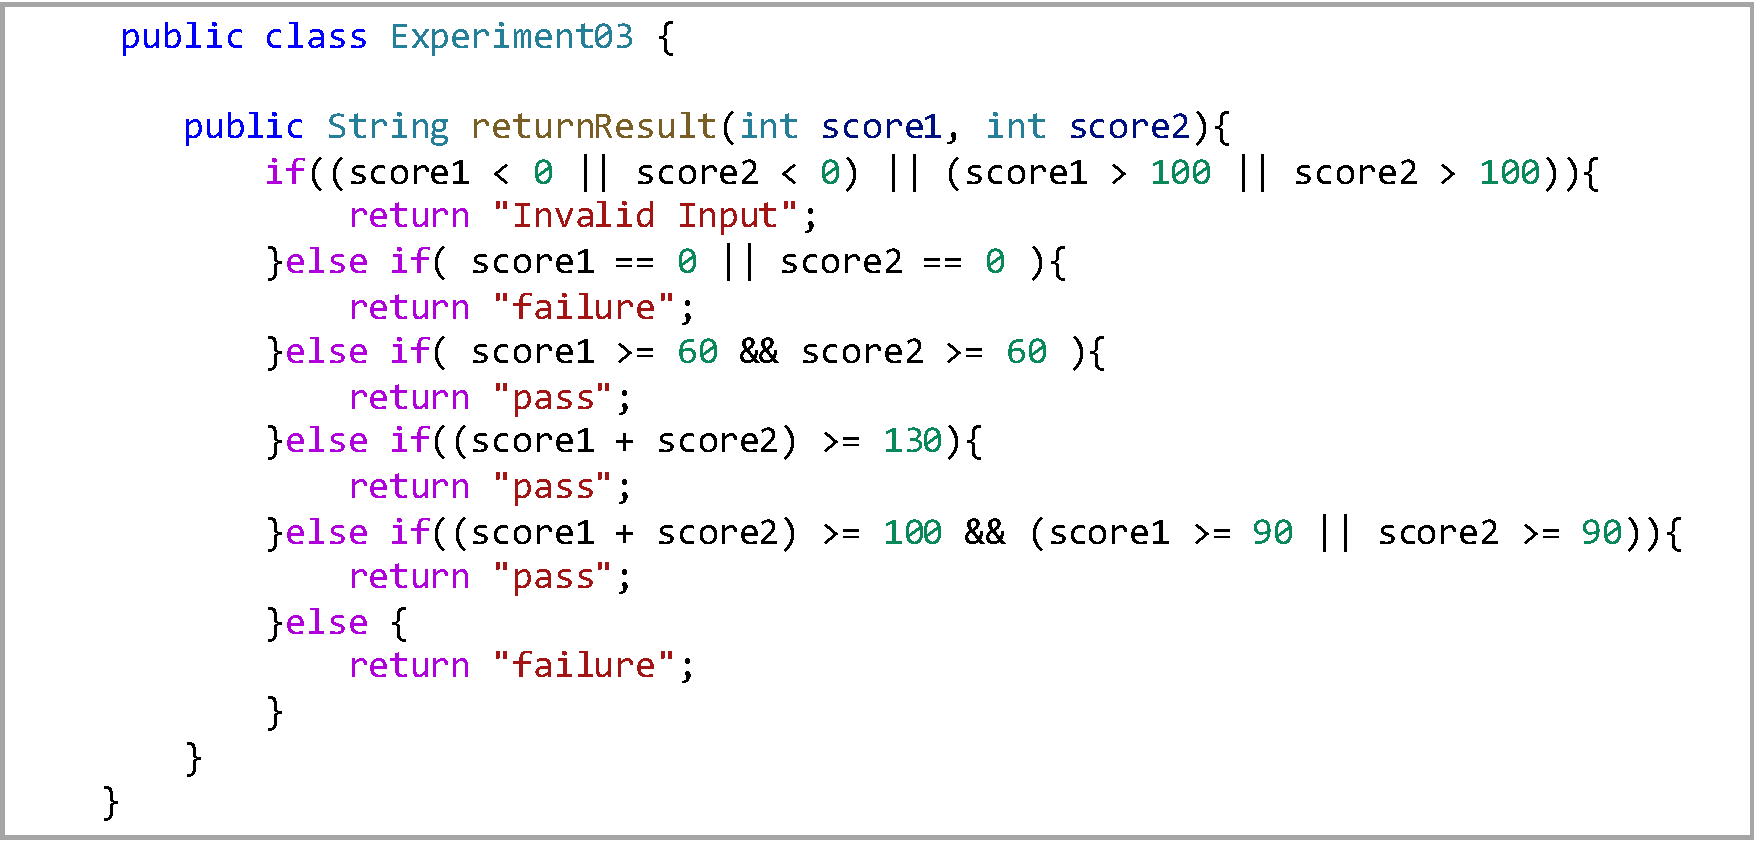
\includegraphics[width=8.9cm]{task.pdf}}
 \caption{Source code of Task 3}
 \label{fig4}
 \end{figure}


The preliminary user study was comprised of two sessions, the tutorial session and the task session. 
In the tutorial session, we gave a quick lecture about basic knowledge about software testing and conducted an exercise of generating JUnit test suites to provide a better understanding of test code generation. The tutorial session has been conducted during 30-minute.
%First, we conducted a 30-minute lecture and practice task on using JUnit from basic knowledge about software testing, and confirmed understanding of the test code description. And we asked them to develop test suites for the three production codes for the actual experiment.

In the task session, we assigned three tasks of creating JUnit test suites to participants with and without \textsf{SuiteRec}. Hereafter, we call each of these assigned tasks as Task 1, Task 2 and Task 3. Task 1 was to generate a JUnit test suite for a java method of FizzBuzz. Task 2 was to generate a JUnit test suite for Java method with four parameters which changes how to calculate three parameters according to the value of the first argument and outputs the result. Task 3 was to generate a JUnit test suite for a Simple Pass/Fail Java method based on the two input values. Among these tasks, Task 3 was relatively difficult compared with Task 1 and Task 2. 
In each task, we provided a production code, targets of generating test suite. Figures \ref{fig4} shows a production code provided in Task 3. The number of conditional branch in the source code used in each task was 8, 16, and 24, respectively. 

We also gave a requirement specification written in natural languages, so that participants could readily the understand the specification of the production code for generating test suite. To mitigate the learning effect of \textsf{SuiteRec}, participants were assigned counterbalanced tasks by dividing into two group. In other words, tasks were conducted with \textsf{SuiteRec} for Task 1, without \textsf{SuiteRec} for Task 2, with \textsf{SuiteRec} for Task 3 in the one group and vice versa. After generating a test suite for each task, participants submitted their test suites. Each participant was given a maximum of 25 minutes to complete each task. At the end of the user study, we conducted a survey to solicit feedback. Survey answers were collected using Google Forms. 



\subsection{Results}
This section presents the results of our user study with answers to four research questions.

\subsubsection{RQ1. How well can \textsf{SuiteRec} support generating test suites with high code coverage?}
%In this experiment, we calculated two types of code coverage: statement coverage (C0) and branch coverage (C1) of test suites submitted by the subjects. To calculate the coverage, we used EclEmma\footnote{https://www.eclemma.org/}, which is installed as a plug-in of the integrated development environment Eclipse\footnote{https://www.eclipse.org/}. Figures \ref{fig5} show the average coverage of statement coverage and branch coverage, respectively. As a result, there is almost no difference in the coverage rate of statement coverage in all three tasks depending on whether SuiteRec is used or not, and the coverage of each task exceeds 90\%.
We answer this RQ with two code coverages, namely statement coverage and branch coverage. To calculate these coverages, we used \textsf{EclEmma}\footnote{https://www.eclemma.org/}, a Java code coverage tool for \textsf{Eclipse}\footnote{https://www.eclipse.org/}.
We compared the average statement coverage and branch coverage of generated test suites with and without \textsf{SuiteRec}. 
Figures \ref{fig5coverage} show the results. In this figure, ``Manual'' indicates the average code coverages of manually written test suites. ``Tool'' indicates the average code coverages created with \textsf{SuiteRec}, respectively. As shown in the figure, Task 1 have the same average code coverage between test suites generated with and without \textsf{SuiteRec}. The average code coverage of test suites generate without \textsf{SuiteRec} are higher in the Task 2, whereas the average code coverage of test suites generate with \textsf{SuiteRec} are higher in the Task 3.
\begin{breakbox}
\textit{Participant generated test suites with higher code coverage, even though the differences were subtle.}
\end{breakbox}


\begin{figure}[htbp]
\centerline{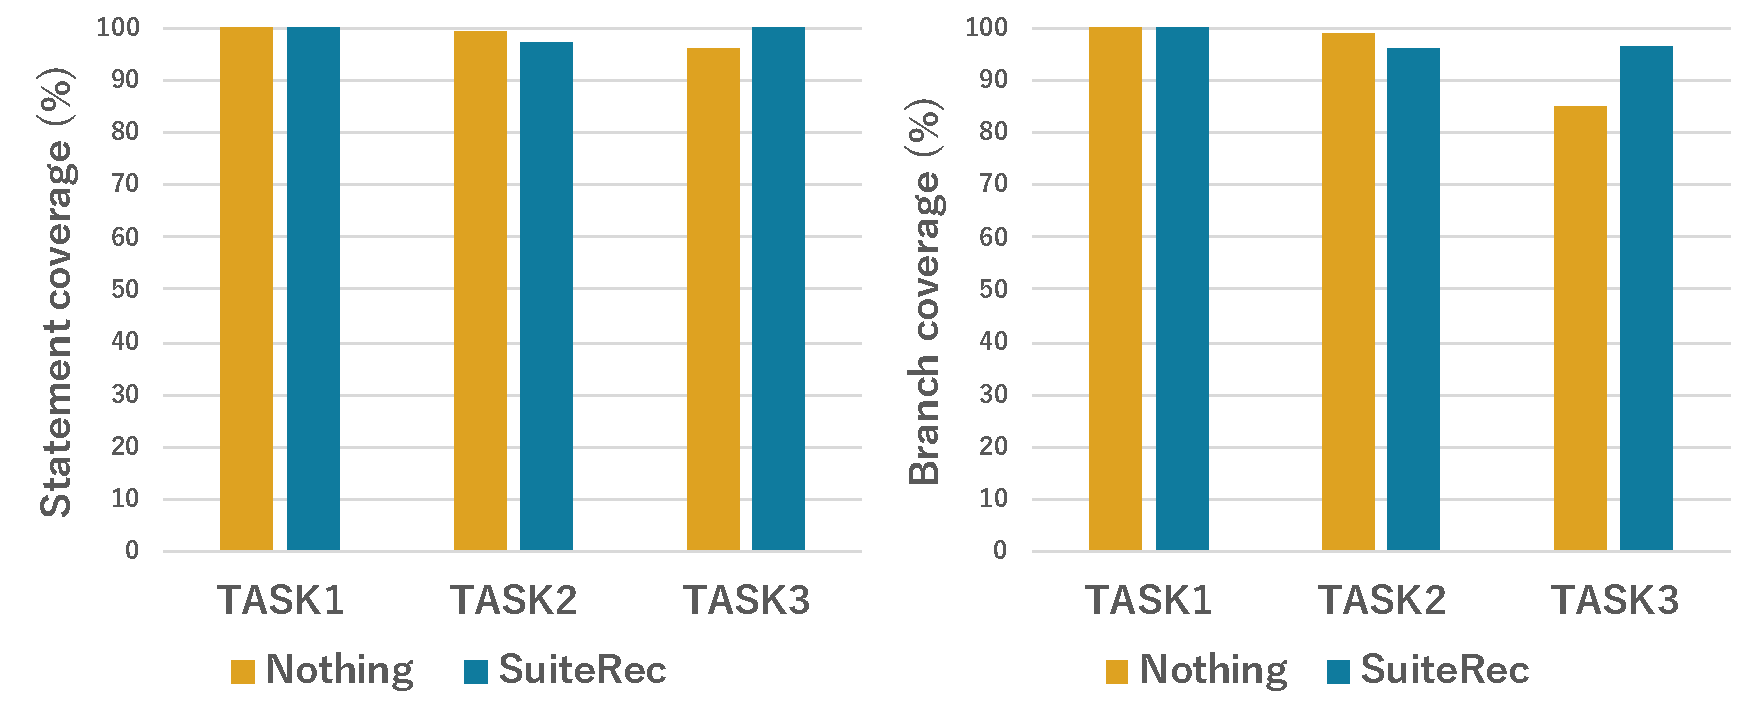
\includegraphics[width=8.6cm]{coverage.pdf}}
\caption{Average code coverage of test suites generated with and without \textsf{SuiteRec}.}
\label{fig5coverage}
\end{figure}

% \begin{figure}[htbp]
% \centerline{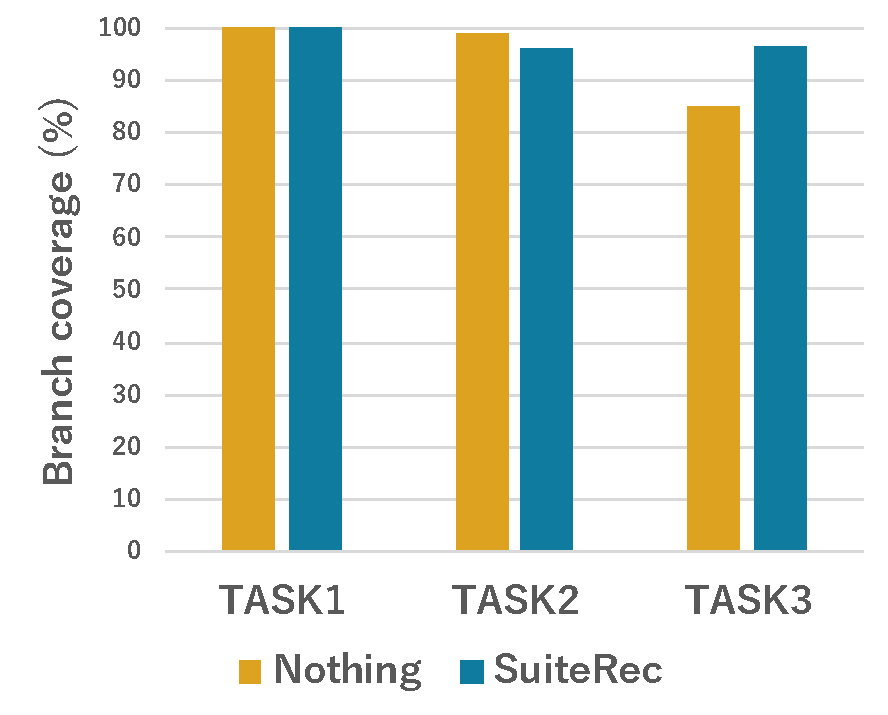
\includegraphics[width=8.5cm]{C1.pdf}}
% \caption{Branch coverage (C1).}
% \label{fig6}
% \end{figure}

\subsubsection{RQ2. How well can SuiteRec reduce test suites generate time?}
We answer this RQ by comparing the time spent completing tasks with and without \textsf{SuiteRec}. Figure \ref{fig7:time} shows the results. As can be seen in this figure, time to generate test suites with \textsf{SuiteRec} took longer in, Task 1 and Task 3. We assume that this is because it took time for participants to read and understand multiple test suites recommended by \textsf{SuiteRec}. In Task 2, time for generating the test with \textsf{SuiteRec} took less. We assumed that this is because participants generated more test cases in the test suites when they generated test suites without \textsf{SuiteRec}.

\begin{breakbox}
\textit{In most cases, it took more time to generate test suites using \textsf{SuiteRec}.}
\end{breakbox}
\begin{figure}[htbp]
\centerline{\includegraphics[width=8.5cm]{time.pdf}}
\caption{Time taken for generating test suites.}
\label{fig7:time}
\end{figure}

\subsubsection{RQ3. How well \textsf{SuiteRec} support generate test code with high quality?}
%Figure \ref{fig8} shows the results of comparing the number of test smells in the submitted test suites with and without SuiteRec. For all tasks, the test codes developed using SuiteRec contains less test smell than if it were not used. This result suggests that the quality of the recommended test codes are high, and the subjects can develop the test codes while maintaining the quality by reusing them. Also, by presenting the test smells included in the recommended test suite, the test code may be rewritten based on it and a high quality test code may have been submitted. %In the actual questionnaire responses, it was reported that the test smells presented were understood and refactored to eliminate them.
%%On the other hand, some subjects were aware that test smells were included, but did not know how to refactor. This is a topic for the future and needs to be improved to show how to refactor test smells.
%As a whole, when SuiteRec was not used, the subjects embedded more than five times the test smells compared to the case where it was used. This is probably because many subjects did not rename the default test method and wrote the Assert statement by copy and paste within one test method. In fact, it has been reported that many of these test smells are detected in existing projects \cite{b9}.
%図6はSuiteRecを使用した場合とそうでない場合で,提出されたテストコード内のテストスメル数を比較しています.すべてのTASKに対して,SuiteRecを使用して作成されたテストコードはテストスメルをあまり含んでいないことが分かる.この結果は,推薦されるテストコード自体の品質が高く開発者はそれを再利用することで品質を維持したままテストコードを作成したと考えられる.また,ツールの出力画面で推薦されるテストスイート内に含まれているテストスメルを提示することで,それを基にテストコードを書き替えより品質が高いテストコードを提出した可能性が考えられる.実際のアンケートの記述でも提示されたテストスメルを理解し,それをなくすようにリファクタリングしテストコードを作成したという報告がされている.一方で,テストスメルが含まれていることは気づいていたがリファクタリングの方法が分からずそのまま提出したと述べている被験者も存在した.これは今後のツールの課題であり,テストスメルのリファクタリング方法も提示する改良の必要がある.SuiteRecを使用しなかった場合は,使用した場合と比べ全体として5倍以上の被験者はテストスメルを埋め込んでいた.その中でも多く埋め込まれていたテストスメルとして,Assertion Roulette, Default Test, Eager Testが挙げられる.多くの被験者は,初期状態のテストメソッドの名前を変更せず一つのテストメソッド内でコピーアンドペーストによってAssert文を記述していたのが原因だと考えられる.実際に既存研究でもこれらのテストスメルが既存プロジェクトで多く検出されていることが報告されている[6]. 


We answer this RQ by comparing the number of test smells in the test suites generated by with tool support and without tool support. Figure \ref{fig8} shows the number of test smells in test suites generated with and without \textsf{SuiteRec}. As can be seen in this figure, the test suites generated with \textsf{SuiteRec} contain less test smells than one that the test suites without \textsf{SuiteRec}. This result indicates participants generated the test suites by reusing high quality test suites recommend by \textsf{SuiteRec}. It also implies participants refer to the test smell information when they selected a target test suite for reusing. Meanwhile, test suites, generated without \textsf{SuiteRec}, contain five times more test smells than test suites generated with \textsf{SuiteRec}. The most frequently occurred test smells were Assertion Roulette, Default Test, and Eager Test. These smells occurred because many participants at first create test code and then wrote the assert statements by copy and paste an existing test code.
\begin{breakbox}
\textit{Participants generated test code with higher quality when using \textsf{SuiteRec}.}
\end{breakbox}


\begin{figure}[htbp]
\centerline{\includegraphics[width=8.5cm]{smells.pdf}}
\caption{Number of detected test smells.}
\label{fig8}
\end{figure}

\begin{figure*}[t]
 \begin{center}
  \includegraphics[width=18.5cm]{qa.pdf}
  \caption{Overview of the survey responses relating to test code generation tasks.}
  \label{fig9}
 \end{center}
\end{figure*}

\subsubsection{RQ4. How effective \textsf{SuiteRec} is to support test suites generation tasks?}
%%%%%%
% Figure \ref{fig9} summarizes answers to the survey questions. Overall, the subjects found the task clear (Question 1), and the allocated time sufficient (Question 2). For the remaining questions, you can see that there is a difference in opinion on the experimental task with and without SuiteRec. 

%Figure \ref{fig9} summarizes answers to the survey questions. When developing test codes, subjects can easily feel test code creation using SuiteRec (Question 1). However, this result contrasts with the actual length of task end time (Figure \ref{fig2}), and it can be seen that the task end time is slower when SuiteRec is used. The subjects read and understand the recommended multiple test suites and determine whether to reuse them. In addition, the test code cannot be applied without modification, and it is necessary to understand the difference between the input code and the detected similar codes and make appropriate modifications to the test codes. We speculate that when using SuiteRec, subjects may spend a lot of time on this part. 

%According to survey SuiteRec improvements, many responses said that it would be better to add functions that support test code editing such as a function that automatically edit classes and methods to names corresponding to the input code. Further improvements in SuiteRec show the potential for reducing the completion time of experimental tasks.

%When using SuiteRec, the subjects are confident in the coverage of the test code developed by themselves (Question 2). On the other hand, 40\% of subjects reported negative responses when nothing was used. However, it is known that there is almost no difference in the coverage of the test code actually submitted (Figure \ref{fig5}). It is important to be confident in the coverage of the test codes they developed. One of the purposes of software testing is that developers are responsible for the code they develop and can provide software to users without anxiety.

%When the test code was developed without using SuiteRec, 40\% of the subjects were not confident in the quality of the test code they wrote (Question 3). It can be seen that the number of test smells in the actual submitted test codes are greater when SuiteRec is not used than when it is used (Figure \ref{fig8}). Developers unknowingly embed test smells that make later maintenance activities difficult. The use of SuiteRec reduces the number of test smells and brings confidence to the code they developed by giving developers an awareness of the quality of the test code.

%On the other hand, even when SuiteRec is used, there are negative opinions about the quality of the test codes. This indicates that developers who are not familiar with test smells may become confused when they were presented with test smells.
%%%%%%%%
We answer this RQ based on the answers to the survey in the user study. Figure \ref{fig9} summarizes answers to three questions from the participants of the user study. From this figure, you can see that participants reported that they felt easier to generate test suites using \textsf{SuiteRec} (Question 1). This is surprised because it took more time for participant to generate test suites using \textsf{SuiteRec} (Figure \ref{fig7:time}). This indicates that participants felt easy to generate the test suites by recommending test suites by \textsf{SuiteRec}, even though it took more time to generate test suites using \textsf{SuiteRec}. Current version of \textsf{SuiteRec} only recommends test suites for reusing, however, we plan to extend \textsf{SuiteRec} to automatically modify existing test suites (e.g., change identifier names and methods names) based on the information of input source code to reduce the test generation time.

 Participants reported higher confidence in the code coverage of test suites when creating test suites using \textsf{SuiteRec} (Question 2). In other words, 40\% of participants reported negatively regarding their confident in the code coverage of test suites generated without tool support. This results were also surprised because there were subtle different in actual code coverage of the test suites generated with and without tool support were very similar (Figure \ref{fig5coverage}). However, the answer to Question 2 indicates that \textsf{SuiteRec} is able to support developers to generate code coverage with confident.

Participants also reported higher confidence in quality of test suites when creating test suites using \textsf{SuiteRec} (Question 3). Meanwhile, 40\% of participants were unsure about the quality of the manually written test suites. This result match with that manually written test suites contains more test smells than test suites generated using \textsf{SuiteRec} (Figure \ref{fig8}). Test smells hinder quality of test code, thus lower the maintainability of test code. The answers to Question 3 indicates that \textsf{SuiteRec} successfully generating high quality test suites reduces the number of test smells and brings confidence to the code by providing the code smell information.

\begin{breakbox}
\textit{Participants felt easy to create test suites with \textsf{SuiteRec}. They also were confident about coverage and quality of test suites generated with \textsf{SuiteRec}.}
\end{breakbox}
 %%%%%%%%%%
% On the other hand, even when SuiteRec is used, there are negative opinions about the quality of the test codes. This indicates that developers who are not familiar with test smells may become confused when they were presented with test smells.
% The respondents reported that they understood Test Smells but didn't know how to refactor. This indicates the need for further improvement of SuiteRec, and we should add the function to present refactoring methods for each test smell.

\subsection{Discussion}
%%%%%
%\subsubsection{Can SuiteRec support test code generation task?}
From Task 1 and Task 3, we observed that participants generated test suites with same or higher code coverage than manually written test suites (RQ1), with longer generation time (RQ2) with \textsf{SuiteRec}. These generated test suites with \textsf{SuiteRec} contain fewer test smells than manually written test suites (RQ3). This implies that even though it took more time to generate test suites with \textsf{SuiteRec}, overall software development cost could be saved by using \textsf{SuiteRec} because manually written test suites have more test smells, indications of a potential problem in the test suites. 

From Task 2, we discovered that participants generated test suites with subtly lower code coverage than manually written test suites (RQ1), with shorter generation time (RQ2) with \textsf{SuiteRec}. These generated test suites with \textsf{SuiteRec} also contain fewer test smells than manually written test suites (RQ3). After analyzing manually written test suites, we found out that higher code coverage and longer generation time of manually written test suites were occurred because they contain redundant test cases. This indicates participants can generate relevant higher quality test cases within shorter time with \textsf{SuiteRec}.

%提示されたテストスメルを理解し,それをなくすようにリファクタリングしテストコードを作成した

In particular, we found that \textsf{SuiteRec} is able to highly contribute to generate high quality test suites. An answer to the free-form questions in the survey seem to corroborate this intuition: {\it ``I could understand the information of test smells by \textsf{SuiteRec} and refactored test suites to eliminate test smells."} Shamshiri et. al.\cite{b1}, reported that developers are less efficient at performing maintenance tasks with generated tests. Meanwhile, participants reported that they felt easy to create test suites and also were confident about coverage and quality of test suites generated using \textsf{SuiteRec} (RQ4). From these results, we believe that developers are efficient at performing maintain tasks with test suites generated with recommendations from \textsf{SuiteRec}.


\section{Related work}
\label{sec:related}
 %Zhang et al. \cite{Zhang:2017} present Grafter, a test reuse and differential testing framework for clones. It transplants one clone to its cloned code by identifying differences between a clone pair, and then the test results before and after transplantation, and reuse the test based on that information.\textit{ Soha [b] et al.} Proposed Skipper that semi-automatically reuses and transforms the relevant part of the test suite corresponding to the code fragment when the developer reuses the code fragment. Skipper's approach is based on Gilligan [10], [34] and requires developers to define a detailed reuse plan to guide the conversion process. SuiteRec differs from these tools in two perspectives. First, SuiteRec searches for similar codes from projects on OSS. It is possible to find many test suites by searching in large projects. Second, SuiteRec only recommends test suites, leaving the detailed test reuse plan between clone pairs to the developer. Even if tests can be reused automatically, spreading low quality code makes maintenance difficult. SuiteRec presents test smells and gives developers confidence in the tests they developed by refactoring themselves.

%a test reuse and differential testing framework for clones, 
Zhang et al. \cite{Zhang:2017} presented Grafter, which transplants one clone to its cloned code to exercise a clone pair using the same test. The results of evaluation of Grafter with 52 clone pairs detected by DECKARD \cite{Jiang:2007} indicate that it successfully reuses tests in 94 \% of clone pairs. Soha et al.\cite{soha:2013} proposed an approach that semi-automatically reuses and transforms test cases from the original test suite. Their approach requires developers to define a detailed reuse plan to guide the conversion process. \textsf{SuiteRec} differs from these approaches in two perspectives. At first, \textsf{SuiteRec} searches for similar codes from projects on OSS projects. Therefore, it provides many test suites by searching in large projects. Second, it only recommends test suites, leaving the detailed test reuse plan between clone pairs to the developer. Even if tests can be reused automatically, spreading low quality code makes maintenance difficult. \textsf{SuiteRec} presents test smells and gives developers confidence in the tests they developed by refactoring themselves.

%\section{Threats to Validity}
%SuiteRec searches similar codes corresponding to the input code from OSS projects and recommends test suites of similar code. Therefore, the test suite cannot be recommended unless a similar code to the input code is found. Even if similar codes can be detected, if the degree of similarity is low, the recommended test suite may not be useful. NICAD detects type 1, type 2 and 3 code clones. Code clones (type 3) with insertion and deletion of statements may behave differently. In such cases, it is difficult to reuse tests. Therefore, the test suites that can be recommended may be limited to a narrow range.

%The main threat of validity is that the recommendations by \textsf{SuiteRec} might be too dependent on the output of \textsf{NiCad} and \textsf{tsDetect}. \textsf{NiCad} detects type 1, type 2 and 3 code clones. Code clones (type 3) with insertion and deletion of statements may behave differently. In such cases, it is difficult to reuse tests. Therefore, the test suites that can be recommended may be limited to a narrow range.

\section{Conclusion and Future Work}
\label{sec:conc}
This paper presents \textsf{SuiteRec}, a recommendation system that finds existing high-quality test codes from OSS projects. \textsf{SuiteRec} finds code clones of the input code from OSS projects and recommends test suites corresponding to the clones. The recommended test suites are ranked by their quality and similarities between the input code and their corresponding source code. Furthermore, test smell information are also shown with test suites.

In the user study, we assigned participants three tasks that generate test suites with and without using \textsf{SuiteRec}. The results indicate that (1) \textsf{SuiteRec} improves code coverage when developing test codes for target codes with many conditional branches, (2) test suites generated with \textsf{SuiteRec} have higher quality and less test smells, and (3) developers felt that it is easier to generate test suites, and they are more confident in the resulting test codes when using \textsf{SuiteRec}.

The followings are future work:

\begin{itemize}
\item \textsf{SuiteRec} needs to provide feature for more practical usage. To do this, we plan to features that automatically modify and refactor test suites.
\item Further evaluation with more participants are necessary. We will conduct an user study with \textsf{SuiteRec} with not not only on students but also practitioners.
\item We need to confirm that current ranking system of \textsf{SuiteRec} is efficient for recommending reusable test suites. To do this, we plan to conduct an extract evaluation about the ranking.
\end{itemize}



\bibliographystyle{IEEEtran}
\bibliography{reference}




\begin{comment}
\vspace{12pt}
\color{red}
IEEE conference templates contain guidance text for composing and formatting conference papers. Please ensure that all template text is removed from your conference paper prior to submission to the conference. Failure to remove the template text from your paper may result in your paper not being published.
\end{comment}
\end{document}
